\documentclass[smallheadings]{scrartcl}

%%% GENERAL PACKAGES %%%%%%%%%%%%%%%%%%%%%%%%%%%%%%%%%%%%%%%%%%%%%%%%%%%%%%%%%%
% inputenc allows the usage of non-ascii characters in the LaTeX source code
\usepackage[utf8]{inputenc}
\usepackage{graphicx}


% title of the document
\title{LGS mit LU Zerlegung}
% optional subtitle
%\subtitle{Draft from~\today}
% information about the author
\author{%
 Aron Ventura und Annika Thiele\\ Humboldt-Universit\"at zu Berlin
}
\date{\today}


%%% LANGUAGE %%%%%%%%%%%%%%%%%%%%%%%%%%%%%%%%%%%%%%%%%%%%%%%%%%%%%%%%%%%%%%%%%%
% babel provides hyphenation patterns and translations of keywords like 'table
% of contents'
\usepackage[ngerman]{babel}

\usepackage[xcolor]{changebar}
\usepackage{lipsum}


\usepackage[color]{changebar}
\cbcolor{red}

\setlength{\changebarsep}{2ex}

\usepackage{amsthm}
\newtheorem{theorem}{Satz}


\theoremstyle{definition}
\newtheorem{definition}{Definition}[section]


%%% HYPERLINKS %%%%%%%%%%%%%%%%%%%%%%%%%%%%%%%%%%%%%%%%%%%%%%%%%%%%%%%%%%%%%%%%
% automatic generation of hyperlinks for references and URIs
\usepackage{hyperref}

%%% MATH %%%%%%%%%%%%%%%%%%%%%%%%%%%%%%%%%%%%%%%%%%%%%%%%%%%%%%%%%%%%%%%%%%%%%%
% amsmath provides commands for type-setting mathematical formulas
\usepackage{amsmath}
% amssymb provides additional symbols
\usepackage{amssymb}
% HINT
% Use http://detexify.kirelabs.org/classify.html to find unknown symbols!

%%% COLORS %%%%%%%%%%%%%%%%%%%%%%%%%%%%%%%%%%%%%%%%%%%%%%%%%%%%%%%%%%%%%%%%%%%%
% define own colors and use colored text
\usepackage[pdftex,svgnames,hyperref]{xcolor}
 
%%% nice tables
\usepackage{booktabs}

%%% Code Listings %%%%%%%%%%%%%%%%
% provides commands for including code (python, latex, ...)
\usepackage{listings}
\definecolor{keywords}{RGB}{255,0,90}
\definecolor{comments}{RGB}{0,0,113}
\definecolor{red}{RGB}{160,0,0}
\definecolor{green}{RGB}{0,150,0}
\lstset{language=Python, 
        basicstyle=\ttfamily\small, 
        keywordstyle=\color{keywords},
        commentstyle=\color{comments},
        stringstyle=\color{red},
        showstringspaces=false,
        identifierstyle=\color{green},
        }

\usepackage{graphicx}
\usepackage{paralist}

\usepackage[style=authoryear, backend=biber,natbib=true]{biblatex}
\addbibresource{LU}

% setting the font style for input und returns in description items
\newcommand{\initem}[2]{\item[\hspace{0.5em} {\normalfont\ttfamily{#1}} {\normalfont\itshape{(#2)}\/}]}
\newcommand{\outitem}[1]{\item[\hspace{0.5em} \normalfont\itshape{(#1)}\/]}
\newcommand{\bfpara}[1]{
	
	\noindent \textbf{#1:}\,}

\begin{document}

% generating the title page
\maketitle
\newpage
% generating the table of contents (requires to run pdflatex twice!)
\tableofcontents
\newpage

%%% BEGIN OF CONTENT %%%%%%%%%%%%%%%%%%%%%%%%%%%%%%%%%%%%%%%%%%%%%%%%%%%%%%%%%%

\section{Einf\"uhrung in die Theorie}
	\subsection{Motivation und Problemstellung}
		Wir beschäftigen uns in diesem Bericht weiter mit dem numerischen Lösen des 
		Poisson Differentialgleichungssystem.  Wir haben bereits gesehen,  dass wir das 
		Poisson Problem numerisch lösen können, indem wir das Gebiet und den 
		Laplaceoperator diskretisieren und so ein lineares Gleichungssystem erhalten.  Um 
		eine gute Approximation zu berechnen,  möchten wir möglichst fein diskretisieren.  
		Mit zunehmender Feinheit,  wächst allerdings auch die Größe der Matrix,  welche 
		das lineare Gleichungssystem darstellt.  Allerdings sind viele Einträge Null. Man 
		spricht hierbei auch von einer sparsen Matrix. Dabei ist unsere bisheriger Ansatz,  
		das Problem mit der LU-Zerlegung zu lösen nicht sehr effizient.  Wir haben 
		gemerkt,  dass die LU-Zerlegung die Sparsität der Gleichungssysteme nicht 
		beibehält. Daher stellt sich die Frage,  wie wir große große (dünnbesetzte) 
		Gleichungssysteme lösen können und die Sparsität für diesen Zweck ausnützen 
		können.  In diesem Bericht beschäftigen wir uns dafür mit einem iterativen 
		Verfahren und vergleichen dieses mit dem Verfahren der LU-Zerlegung. Wir 
		ziehen dabei sowohl den Speicherbedarf als auch den Rechenaufwand in 
		Betracht. 
	\subsection{Theoretischer Hintergrund}
	
	\subsubsection{Poisson Problem}
		 \cbstart Wir definieren den Laplace Operator wie in \citep{PDE}.
		\begin{definition}[Laplace Operator]
		Der Laplace Operator einer Funktion $u\in C^2(\mathbb{R}^d,\mathbb{R})$ ist definiert durch
		$$\Delta u=\sum_{i=1}^d\frac{\partial ^2 u}{\partial x_i^2}$$

		\end{definition}
		Wir definieren weiter das partielle Differentialgleichungssystem wie in \citep{PDE}, welches im Poisson-Problem gelöst werden soll. Wir betrachten das Problem auf einem  Gebiet  $\Omega$ und Rand $\partial \Omega$. seien $f\in C(\Omega , \mathbb{R})$ und $g\in C(\partial \Omega , \mathbb{R})$ Funktionen. Dann suchen wir eine Funktion $u$, sodass
		\begin{align*}
		\Delta u&=f \text{ in }\Omega\\
		u&= g \text{ auf }\partial\Omega
		\end{align*}
		Wir betrachten in diesem Bericht einen Spezialfall des Problems, wo $\Omega =(0,1)^d$, $d\in \{1,2,3\}$ und $g\equiv 0$

		Wir wollen das Problem numerisch mit \textit{Finiten-Differenzen} approximieren. Nach \citep{finite}
		\begin{definition}[Finite-Differenzen-Methode]
		Finite-Differenzen-Methoden sind eine Klasse numerischer Verfahren zur Lösung gewöhnlicher und partieller Differenzialgleichunen.		
		Die grundlegende Idee bei der \textit{Finite-Differenzen-Methode} ist es die Ortsableitung in der Differenzialgleichung an einer endlichen Zahl Gitterpunkten durch Differenzenquotienten zu approximieren. Unsere angenäherten Lösungen der Differenzialgleichung an den Gitterpunkten führen dann auf ein entsprechendes Gleichungssystem, welches sich numerisch berechnen lässt.
		\end{definition}
		In unserem Fall diskretisieren wir dazu das Gebiet $\Omega$ und den Laplace Operator durch \textit{Finite Differenzen} um ein lineares Gleichungssystem zu erhalten.
		 Im Folgenden wird die Theorie hinter unserem Verfahren zum numerischen lösen des Problems nach \citep{PDE}, \citep{Wiki}. Wir diskretisieren das Gebiet indem wir das Intervall $(0,1)$ in $n$ äquidistante Teilintervalle zerlegen. Die so entstehenden Gitterpunkte im $(0,1)^d$ werden unsere Diskretisierungspunkte. Mit den Finiten Differenzen zweiter Ordnung können wir den Laplace Operator diskretiseren, denn wir wissen aus \citep{Wiki}, dass 
		$$\frac{\partial^2u}{\partial x_l^2} \approx D_h^{(2)} u_{x,l}(x) =\frac{u(x_1,...,x_l+h,...,x_d) - 2u(x_1,...,x_l,...,x_d) + u(x_1,...,x_l-h,...,x_d)}{h^2}$$
		gilt. 
		Um ein lineares Gleichungssystem zu erhalten, definieren wir eine Ordnung auf den Diskretisierungspunkten.
		
		\begin{definition}
		Seien $x=(x_1,...,x_d)$ und $y=(y_1,...,y_d)$ zwei Diskretisierungspunkte. Dann gilt $x <_X y$ genau dann, wenn
		$$\sum_{l=1}^dx_ln^l<\sum_{l=1}^dy_ln^l$$
		\end{definition}
		Sei $N:=(n-1)^d$ die Anzahl an Diskretisierungspunkten.
		So erhalten wir $N$ lineare Gleichungen und damit Blockmatrizen $A^{(d)}$, für die zu lösen gilt $A^{(d)}\hat{u}=b$. Wir definieren diese Blockmatrizen induktiv.
		$$A^{(d)}_{1} := \begin{pmatrix}     2d & -1 & 0 & 0 &\dots&0 \\    -1 & 2d & -1 & 0&\dots&0 \\    0&\ddots&\ddots&\ddots&\ddots&\vdots\\    \vdots & \ddots &\ddots&\ddots&-1&0 \\    0 & \dots&0&-1&2d&-1\\     0&  \dots&0&0&-1&2d    \end{pmatrix}$$
		$$A^{(d)}_{l} := \begin{pmatrix}     A^{(d)}_{l-1} & -\mathbf{I}_{l-1} & 0 & 0 &\dots&0 \\    -\mathbf{I}_{l-1} & A^{(d)}_{l-1} & -\mathbf{I}_{l-1} & 0&\dots&0 \\    0&\ddots&\ddots&\ddots&\ddots&\vdots\\    \vdots & \ddots &\ddots&\ddots&-\mathbf{I}_{l-1}&0 \\    0 & \dots&0&-\mathbf{I}_{l-1}&A^{(d)}_{l-1}&-\mathbf{I}_{l-1}\\     0&  \dots&0&0&-\mathbf{I}_{l-1}&A^{(d)}_{l-1}    \end{pmatrix}$$
		Wir setzen $A^{(d)}:=A^{(d)}_d$ Die rechte Seite $b$ erhalten wir durch das Einsetzen der Diskretisierungspunkte in die gegebene Funktion $f$. \cbend
		\subsubsection{LU Zerlgeung}
		Wir haben im letzten Bericht die LU-Zerlegung einer Matrix genutzt um das Poisson Problem diskret zu lösen. 
		Bei der LU-Zerlegung wird eine Matrix $A$ wird diese Matrix in eine  oberen rechten Dreiecksmatrix mit Einsen auf der Hauptdiagonalen und einer unteren linken Dreicksmatrix zerlegt.  Danach kann ein Gleichungssystem durch Rückwärts und Vorwärtseinsetzen gelöst werden.  
		\subsubsection{Iterative numerische Verfahren}
			Im Vergleich zu dem Verfahren zum lösen linearer Gleichungssysteme 
			mit der LU-Zerlegung,  enden iterative numerische Verfahren nicht nach
			endlich vielen Schritten mit einer exakten Lösung, sonder nähern sich vielmehr 
			Schrittweise an die genaue Lösung an.  Wie wir gesehen haben, kommt es 
			auch bei dem exakten Lösen des Problems zu Fehlern.  Daher ist es sinnvoll
			sich anzuschauen, ob man mit iterativen Verfahren mit weniger Aufwand
			und Speicherbedarf zu einer ähnlich gut approximierten Lösung
			kommen kann.  Dass ein solches Iterationsverfahren konvergiert auf
			Grundlage des Banachschen Fixpunktsatzes.
			Wir definieren zunächst wie in \citep{kont}
			\begin{definition}[Kontraktion]
			Sei $(X,d)$ ein metrische Raum.  Eine Abbildung $f:X\rightarrow X$ heißt 
			\textit{Kontraktion}, wenn sie Lipschitz stetig ist mit einer Lipschitzkonstanten
			$0\leq \lambda < 1$,  es also für alle $x,y\in X$ gilt:
			$$d(f(x),f(y))\leq \lambda d(x,y)$$
			\end{definition}
			Die Aussage des folgenden Satzes beruht auf \citep{ban}
			\begin{theorem}[Banachscher Fixpunktsatz]
			Sei $(X; d)$ ein vollständiger Metrischer Raum.  Sei $A\subset X$ 
			abgeschlossen und nicht-leer. Sei $f:A\rightarrow A$ eine Kontraktion. Definiere
			eine Folge $(x_n)$ mit beliebigen Startwert durch 
			$$x_{n+1}=f(x_n)$$
			Dann existiert genau ein Fixpunkt von $f$.  Dieser ist der Grenzwert von 
			$(x_n)$.
			\end{theorem}
			Wir betrachten ein lineares Gleichungssystem $Ax=b$ für eine Matrix
			$A\in \mathbb{R}^{m\cross m}$ Unser Iterationsansatz von \citep{skript}
			 $$x_{n+1}=Bx_n+d$$
			 für geeignet gewähltes $B$ und $d$,  konvergiert nach dem Banachschen 
			 Fixpunktsatz, wenn die rechte Seite als Abbildung eine 
			 Kontraktion ist. 
			Wir werden uns in diesem Bericht ein spezielles Splitting Verfahren genauer
			anschauen.  Allgemein zerlegt man bei Splitting Verfahren wie in \citep{skript}
			beschrieben die Matrix $A=M+N$ in eine Summe von Matrizen und wählt dann
			$$B:=-M^{-1}N,  \text{ } d=M^{-1}b.$$
			Es wird in \citep{skript} gezeigt, dass die Iteration mit genau dann eine
			Kontraktion ist und somit konvergiert, wenn 
			$\rho (B):=\max_{1\leq i \leq m} |\lambda _i(B)|<1$ gilt.
			Wir betrachten folgende Zerlegung von $A$ in die Summe einer unteren
			Dreiecksmatrix, einer Diagonalmatrix und einer oberen Dreiecksmatrix.
			\begin{definition}
			Sei $A\in \mathbb{R}^{m\cross m}$.  Wir definieren die Matrizen
			$$A=L+D+U:=\begin{pmatrix}
			0&0&\hdots &0\\
			*&0&\hdots &0\\
			\vdots &&\ddots &\vdots\\
			*&*&\hdots &0
			\end{pmatrix}+\begin{pmatrix}
			*&0&\hdots &0\\
			0&*&\hdots &0\\
			\vdots &&\ddots &\vdots\\
			0&0&\hdots &*
			\end{pmatrix}+\begin{pmatrix}
			0&*&\hdots &*\\
			0&0&\hdots &*\\
			\vdots &&\ddots &\vdots\\
			0&0&\hdots &0
			\end{pmatrix}$$
			
			\end{definition}
			
			Dann betrachten wir für das sogenannte \textbf{SOR-Verfahren (Successive 
			Over Relaxation} wie auch in \citep{skrpit} die Zerlegung  mit
			$M:=L+\frac{1}{\omega}$ und $N:=U-(\frac{1}{\omega} -1)D$,  also die 
			Iteration 
			\begin{align}\label{sor_iteration}
			x_{n+1}=\omega (-D^{-1}Ux_n-D^{-1}Lx_{n+1}+D^{-1})+(1-\omega )x_n
			\end{align}
			für ein geeignetes $\omega$.
			Wir bekommen also eine Iterationsmatrix wie in \citep{konvergenz}
			\begin{align*}
			M_{SOR}(\omega )=(D-\omega L)^{-1}[(1-\omega)D+\omega U].
			\end{align*}
			Angelehnt an \citep{konvergenz}, können wir zeigen,  dass das SOR Verfahren nur konvergiert für $\omega \in (0,2)$. Das liegt am folgenden Satz aus \citep{kovergenz}
			
			\begin{theorem}[Satz von Kahan]
			Für jede Matrizen $A\in \mathbb{R}^{n\times n }$ mit regulärem Diagonalteil $D$ gilt 
			\begin{align}\label{omegabetween02}
			\rho (M_{SOR} )\geq |\omega -1|
			\end{align}
			\end{theorem}
			
			
			
			Da wir bei iterativen Verfahren nicht nach endlich vielen Schritten zu einer
			exakten Lösung kommen,  möchten wir das Verfahren bei einer gewissen
			Genauigkeit der Lösung abbrechen.  Dafür geben wir einen Wert $\varepsilon$ 
			an, und setzen die Abbruchbedingung als $$||Ax_i-b||<\varepsilon$$ für $x_i$ 
			als Lösung des $i$-ten Iterationsschrittes.  
			
		\subsubsection{Rechenaufwand und Speicherplatz}	
		
		Im Gegensatz zum Verfahren mit der 
		LU-Zerlegung,  benötigen wir in dem oben beschriebenen Iterativen Verfahren 
		nicht mehr Speicherplatz, denn die Anzahl an Nicht-Null Eintägen der Zerlegung 
		ist genauso groß wie die der Matrix $A$. Das liegt daran, dass wir die Matrix $A$ für das Verfahren aufteilen in $A=L+D+U$, wobei aber wenn man $L,D,U$ in eine Matrix abspeichert genau $A$ rauskommt. Daher ist die Anzahl an Nicht-Null Einträgen gleich zu der von der Matrix $A$. Bei der LU Zerlegung hingegen ist die Anzahl an Nicht-Null Einträgen in der LU Zerlegung im Allgemeinen größer als die von $A$.
		
		Der Rechenaufwand von dem SOR-Verfahren ist in jedem Schritt nach
		 \citep{slides} linear beschränkt, also in $\mathcal{O}(n)$, für eine 
		 dünnbesetzte Matrix $A\in\mathbb{R}^{n\cross nm}$.  
		 
		 \subsubsection{Optimaler Wert $\omega$}
		 Der optimale Relaxationswert $\omega$ ist sehr Problemabhängig. Für das Poisson Problem ist er nach \citep{slides} bekannt und beträgt
		 \begin{align*}
		 \omega _{opt}:=\frac{2}{1+\sqrt{1-\mu ^2}}
		 \end{align*}
		 wobei $\mu$ der Spetralradius von $I-D^{-1}A$ ist, also 
		 \begin{align*}
		 \mu = \rho (I-D^{-1}A).
		 \end{align*}
		 
		 
		
\section{Implementierung}

\texttt{solve\_ sor()}

\subsubsection*{Bedienungshilfe \texttt{linear\_solvers.py}}
In \texttt{linear\_solvers.py} ist eine \texttt{main()} Funktion implementiert. Sie dient zur Demonstration ausgewählter vorhandender Funktionen und
		wird nur ausgef\"uhrt wenn \texttt{linear\_solvers.py} direkt mittels \texttt{python3 linear\_solvers.py} gestartet wird. 
Die \texttt{main()} stellt die Funktionalität von \texttt{solve\_sor()} vor. Zunächst kann vom Nutzer die Parameter $3\geq n\geq 15$ und $1\geq d\geq 3$ ausgewählt werden. Wird bei einer der Eingaben kein \textit{Integer} angegeben wird eine \texttt{ValueError}-Exception geworfen.
Es wird die Koeffizienenmatrix $A$ zu den gegebenen Werten $n$, $d$  erstellt. Um für $b$ ein Array in der passenden Form zu erhalten nehmen wir $[1,\cdots,1]$.
Das Programm gibt dann die Lösung $x$ zur Gleichung $Ax=b$ aus sowie das Residuum zur gefundenen Lösung.

\subsection*{Bedienungsanleitung \texttt{experimente\_it.py}}
\texttt{experimente\_it.py} besitzt eine \texttt{main()} Funktion, welche unsere Experimente vorstellen kann. Dabei kann der Nutzer selbst wählen welches Experiment durchgeführt werden soll.
Dazu werden die möglichen Experimente aufgelistet, zusammen mit einer Zahl. Die zugehörige Zahl zum Experiment, das gesehen werden soll, muss danach eingegeben werden. Wird eine andere Eingabe eingegeben, wird der Nutzer darauf hingewiesen und nochmal um eine Eingabe gebeten. Nach dem Auswählen eines Experimentes, wird dieses durchgeführt.
Wird bei einer der Eingaben kein \textit{Integer} angegeben wird eine \texttt{ValueError}-Exception geworfen.\\
\\

\bfpara{\textit{1: Plot zum Fehler des iterativen Verfahrens}}\\
Es wird ein Plot betrachtet, der für Dimension $=1,2,3$ den Fehler für die Iterationen zeigt. Der Nutzer
kann hierbei ein $n$ zwischen $3$ und $18$ wählen.
\bfpara{\textit{2: Plot zu unterschiedlichen Epsilon als Abbruchkriterium}}\\
Der Nutzer wählt das maximale $3\geq n\geq 47$. Dann wird ein Plot mit Schrittweite $5$
erstellt, mit dem man den Fehler der Lösung für unterschiedliche Epsilon vergleichen kann.
Epsilon sind hierbei $h^k$($h=\frac{1}{n}$) mit $k=-2,0,2,4,6$.
\bfpara{\textit{3: Plot zum Fehler in Abhängigkeit von Omega}}\\
Diese Funktion illustriert den Fehler in Abhängigkeit von Omega für $d=2$ und ein vom Nutzer gewähltes
$3\geq n\geq 15$.
\bfpara{\textit{4: Plot zum Fehler des SOR- und des LU-Verfahrens}}\\
Zunächst kann der Nutzer ein $n$ zwischen $3$ und $40$ auswählen.
Diese Funktion erstellt einen Graphen, der für $d=1$ das Konvergenzverhalten
des LU und SOR-Verfahrens vergleicht. Das SOR-Verfahren läuft
einmal mit \texttt{max_iter}$=3000$ und einmal mit \texttt{max_iter}$=10000$. Es wird außerdem \texttt{omega}$=0.1$ verwendet.
\bfpara{\textit{5: Vergleich der Laufzeit des SOR- und des LU-Verfahrens}}\\
    Der Nutzer wählt ein $3\geq n\geq 10$ und für die Dimension verwenden wir $d=1$.
    Diese Funktion erstellt einen Graphen, der die Laufzeit des
    LU- und des SOR-Verfahrens komponentenweise und mit
    solve-triangular vergleicht. Hierfür wird für jeden Punkt die Funktion $15$ mal durchlaufen und dann der Mittelwert gebildet.
\bfpara{\textit{6: Vergleich der Sparsität der beiden Verfahren}}\\
Hier wird die Anzahl Nicht-Null-Einträge der Matrizen mit und die der korrespondierenden LU-Zerlegung einander gegenüber gestellt.

\section{Beschreibung der Experimente}

 \cbstart Im Rahmen unserer Experimente werden wir uns mit folgender Funktion beschäftigen.
Sei $u:\Omega\rightarrow \mathbb{R}$ definiert durch
$$u(x):=\prod_{l=1}^dx_l\sin (\pi x_l)$$
Wir berechnen

$$f(x)=\Delta u= \sum_{i=1}^d\frac{\partial ^2 u}{\partial x_i^2}=
 \sum_{i=1}^d \left(\prod_{l\neq i}x_l\sin (\pi x_l)\right)\left(-x_i\pi ^2\sin (\pi x_i)+(1+\pi)\cos (\pi x_i) \right)$$

Dann ist $u$ die exakte Lösung zum Poisson Problem mit $f$ wie oben definiert. Wir können also nun numerisch das Poisson Problem lösen und das Ergebnis mit $u$ vergleichen um den Fehler zu erhalten. \cbend
\subsection{Fehleranalyse}
Wir schauen uns zunächst an, wie sich der Fehler im Laufe der Iterationen verhält. Dazu betrachten wir die folgende Abbildung \ref{error}, in der der maximale absolute Fehler der Iterierten für $d\in\{1,2,3\}$ und $27$ Diskretisierungspunkten.  




\begin{minipage}{\textwidth}

 \centering
 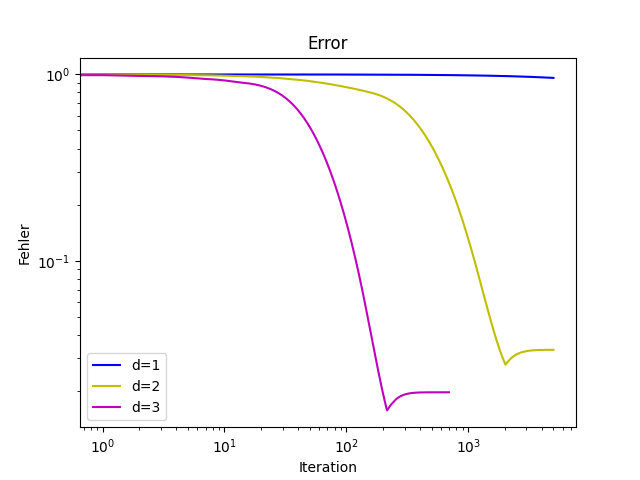
\includegraphics[scale = 0.9]{Error1}
 	\captionof{figure}{Fehleranalyse}
 	\label{error}

 \end{minipage}
 
 Diese Grafik ist doppelt-logaritmisch skaliert. 


\subsection{Konvergenzverhalten mit verschiedenen Abbruchbedingungen}
Wir untersuchen das Konvergenzverhalten, je nachdem, welchen Wert man als Abbruchbedingung wählt.  Wir variieren in der folgenden Abbildung \ref{epsilon} das $\varepsilon$,  zu welchem die Abbruchbedingung $||Ax_i -b||<\varepsilon$ genutzt wird. Wir schauen uns an, wie der maximale absoluter Fehler sich in ABhängigkeit von $n$ verhält. 


\begin{minipage}{\textwidth}

 \centering
 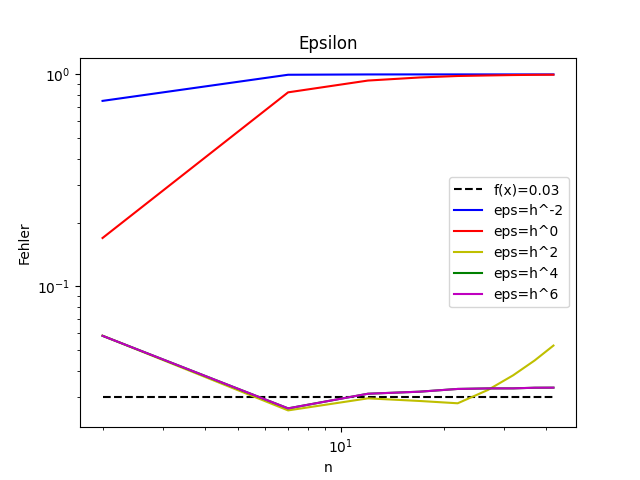
\includegraphics[scale = 0.9]{epsilon1}
 	\captionof{figure}{Vergleich von versdchiedenen Abbruchbedingungen}
 	\label{epsilon}

 \end{minipage}
 
 Man erkennt, dass mit kleinerem $\varepsilon$ ist auch der Fehler geringer, so sind die Fehler für $\varepsilon =\frac{1}{n^{-2}}$ und $\varepsilon =1$ für größere $n$ ungefähr Eins.    Für $\varepsilon =\frac{1}{n^{2}}$ ist der Fehler schon viel kleiner und für  $\varepsilon =\frac{1}{n^{4}}$ und  $\varepsilon =\frac{1}{n^{6}}$ ist der Fehler ähnlich aber noch kleiner.  Durch die eingezeichnete Hilfsgeraden kann man sehen, dass mit zunehmenden $n$, der Fehler sich ab $n=10$ nicht mehr viel ändert.  Bei $\varepsilon = \frac{1}{n^{-2}}$ sieht man bei höheren $n$, dass auch der Fehler wieder steigt.

\subsection{Experimentelle Ermittlung des optimalen Relaxationsfaktor $\omega$}
Je nachdem welchen Relaxationsfaktor man für das SOR-Verfahren nutzt,  bekommt man unterschiedlich genaue Lösungen.  In der Theorie haben wir bereits gesehen, dass der optimale Wert für $\omega$ beträgt.  Wir werden das nun experimentell überprüfen.  Dazu ist in der folgenden Grafik \ref{omega}
 der Fehler in Abhängigkeit von dem verwendeten Relaxationsfaktor aufgetragen.  Es ist hier der Fehler von der durch das SOR Verfahren erhaltenen Lösung für $n=11$, $d=2$ mit den Abbruchbedingungen wie in Abbildung \ref{error} für verschiedene $\omega$ berechnet. Wir ziehen Werte $\omega \in (0,2)$ in Betracht, da das Verfahren nach \ref{omegabetween02} sonst nicht konvergiert.

\begin{minipage}{\textwidth}

 \centering
 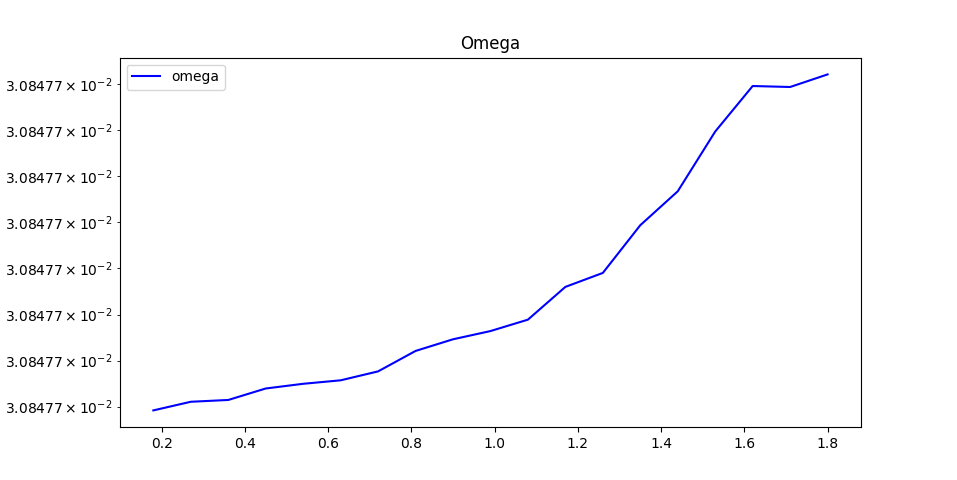
\includegraphics[scale = 0.5]{Omega1}
 	\captionof{figure}{Optimaler Relaxationswert}
 	\label{omega}

 \end{minipage}
		 
	Hier ist zu sehen, dass mit zunehmendem Relaxationswert, auch der Fehler zunimmt. 
	
		
\subsection{Vergleich LU und SOR}
\subsubsection{Konvergenzverhalten}

Wir betrachten für die Dimensionen $d=2$ die approximierte Lösung der Poisson-Gleichung durch das LU- und das SOR-Verfahren für verschiedene  $n$ an.   Wir schauen uns den Fehler beim SOR Verfahren für feste Abbruchbedingungen an,  entweder wenn $||Ax_i-b||-||Ax_{i+1}-b||<10^{-7}$, $||Ax_i-b||<10^{-8}$ oder wenn die maximale Iterationszahl überschritten ist.  In der folgenden Abbildung,  sind die Fehler der Lösungen des Poisson Problems mit durch die beiden Verfahren in Abhängigkeit von $n$ geplottet.




\begin{minipage}{\textwidth}

 \centering
 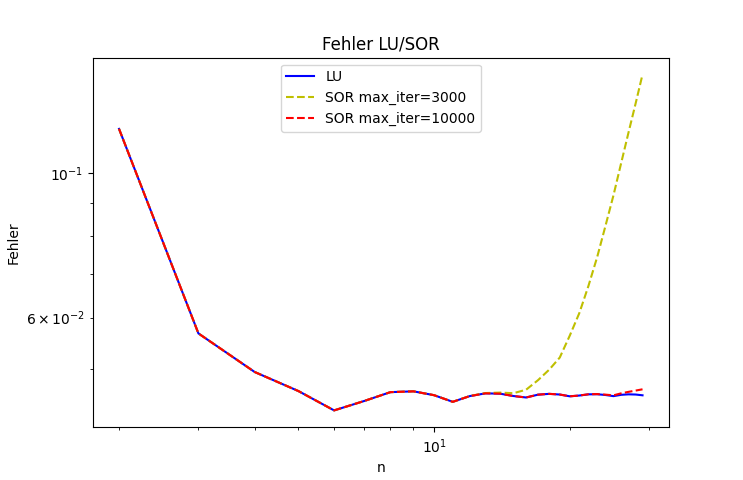
\includegraphics[scale = 0.8]{Errorlu1}
 	\captionof{figure}{Vergleich von dem Fehler}
 	\label{errorcomp}

 \end{minipage}
 
 Wir sehen in dem Graphen, dass der Fehler beim Lösen des Differentialgleichungssystems durch das LU und durch das SOR Verfahren für die gewählten Werte gleich ist.  Man erkennt aber hier gut den Einfluss von der maximalen Iterationszahl, denn ab $n>10$ wächst der Fehler der Lösung durch das SOR Verfahren mit einer kleineren maximalen Iterationsszahl stark an.
 
 

\subsubsection{Sparsität}
Bei dem Poisson Problem betrachten wir sehr dünnbesetze aber große Matrizen.  Beim Speichern ist es daher sinnvoll nur die Nicht-Null Einträge und deren Position zu betrachten.  Wir haben im letzten Bericht gesehen,  dass die LU Zerlegung im Allgemeinen mehr Nicht-Null EInträge besitzt als die ursprüngliche Matrix $A$.  Beim SOR Verfahren hingegen erhält man durch das \textit{splitting} von $A=L+D+U$ drei Matrizen mit gleich vielen Nicht-Null Einträgen.  Wählt man eine sehr feine Diskretisierung des Gebietes für das Poisson Problem,  so benötigt man also mit dem SOR Verfahren weniger Speicherplatz.   Experimentell überprüfen wir dies, indem wir für verschiedene $N$, der Anzahl an Diskretisierungspunkten, die Sparsität vergleichen. 
In der folgenden Abbildung \ref{sparsity} ist in Abhängigkeit von $N$ die relative Sparsität, also Anzahl an Nicht-Null Einträgen aufgezeichnet. 

\begin{minipage}{\textwidth}

 \centering
 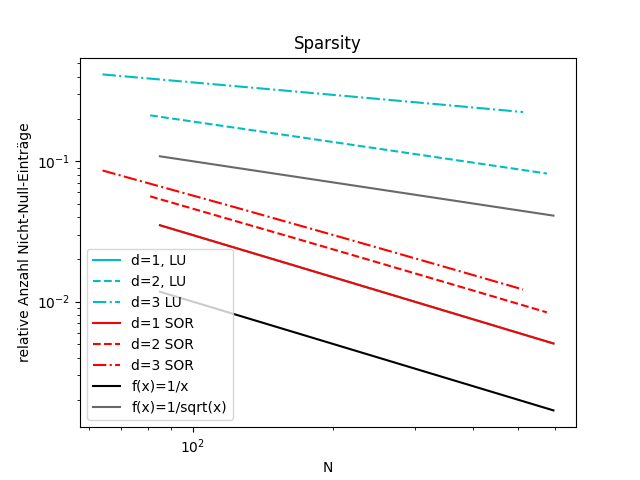
\includegraphics[scale = 0.9]{Sparsity1}
 	\captionof{figure}{Vergleich von Sparsität}
 	\label{sparsity}

 \end{minipage}

Man kann erkennen, dass die relative Anzahl der Nicht-Null Einträge im SOR Verfahren schneller abnimmt, als die der LU Zerlegung.  Es ist zu beachten, dass diese Abbildung doppelt-logarithmisch  skaliert ist.  Durch die eingezeichneten Hilfsgeraden sieht man, dass die Geraden des SOR Verfahrens parallel zur Funktion $f(x)=\frac{1}{x}$. Die Geraden der LU Zerlegung haben verschiedene Steigungen,  je nachdem welche DImension betrachtet wird. Bei Dimension $d=1$ gibt es keinen Unterschied zwischen der Sparsität der LU-Zerlegung und der Matrix beim SOR Verfahren.  Bei Dimension $d=2$ hingegen, verläuft die Gerade parallel zur Hilfsgeraden zur Funktion $f(x)=\frac{1}{\sqrt{x}}$. 

\subsubsection{Laufzeit}
Um die beiden Verfahren hinsichtlich der Laufzeit zu vergleichen,  messen wir jeweils für $d=2$ und verschiedene $n$ die Zeit, welche die jeweiligen Verfahren benötigen um das Poisson Problem zu lösen.  Um Störungen auszugleichen,  nehmen wir den Mittelwert von mehreren Messungen.Für das SOR Verfahren vergleichen wir zusätzlich eine weitere Implementation,  welche das SOR Verfahren komponentenweise ausführt. 



\section{Auswertung der Experimente}
\section{Zusammenfassung}

Im Gegensatz zu direkten Verfahren, nähert man sich bei iterativen Verfahren an die exakte Lösung mit jeder Iteration weiter an.  Wir haben uns hier ewin spezielles Iterationsverfahren angeschut, nämlich das SOR-Verfahren. Wir haben in unseren Experimenten diese im Hinblick auf Konvergenzverhalten, Laufzeit und Sparsität untersucht und mit dem LU-Verfahren, ein direktes Verfahren zur Lösung linearer Gleichungssysteme, verglichen.  Wir haben gesehen, dass man durch das iterierte Verfahren schneller und effizienter zu einer sehr genauen Lösung kommt.  Das liegt zum einen an einem niedrigeren Rechenaufwand, und zum anderen wird weniger Speicherplatz benötigt als beim LU-Verfahren. 

\section{Ausblick}
Wir haben in diesem Bericht uns die Vor und Nachteile der beiden Verfahren, zum einen dem LU-Verfahren und zum Anderen dem SOR-Verfahren, angeschaut.  Allerdings ist es in der Anwendung in der Regel nötig,  sehr feine Disretisierungen anzuschauen, und eine möglichst gute Approximation zu erhalten.  Es resultieren riesige Lineare Gleichungssysteme. Daher ist es sinnvoll, sich noch effizientere Iterationsverfahren als das SOR Verfahren anzuschauen. In der Literatur gibt es sehr viele verschieden. Im Weiteren Studium über das numerische Lösen von Gleichungssystemen kann man also die Vor und Nachteile der optimierteren iterierten Verfahren anschauen. 



\printbibliography

%%% END OF DOCUMENT %%%%%%%%%%%%%%%%%%%%%%%%%%%%%%%%%%%%%%%%%%%%%%%%%%%%%%%%%%%
\end{document}
